\documentclass[9pt,twocolumn,twoside]{gsag3jnl}

\articletype{inv} % article type

\usepackage{bm}
\usepackage{tabu}
\usepackage{graphicx}
\usepackage{caption}
\usepackage{subcaption}

\newcommand{\T}{^\text{T}}
\newcommand{\N}{\text{N}}
\newcommand{\twolinecell}[2][c]{%
  \begin{tabular}[#1]{@{}c@{}}#2\end{tabular}}
\graphicspath{{images/}}

\newcommand{\redstar}{\textcolor{red}{*}}


\title{\texttt{vqtl}: An \texttt{R} package for QTL Mapping on Phenotypes with Heterogeneous Variance}

\author[$\ast$]{Robert W. Corty}
\author[$\ast, 1$]{William Valdar}
\affil[$\ast$]{Department of Genetics, University of North Carolina at Chapel Hill}


\keywords{QTL mapping, variance heterogeneity}
\runningtitle{R package vqtl} % For use in the footer
\correspondingauthor{Robert Corty}
\setboolean{displaycopyright}{true}

\begin{abstract}
Existing methods for QTL mapping in experimental crosses assume that the amount of residual variation is constant across all individuals.
Many common situations violate this assumption.
For example, female mice often have more variable phenotypes than males, some experimenters make more precise measurements than others, and specific genetic loci may influence the extent of variation between individuals.
In all such cases, the heterogeneous variance modeling approach demonstrated here provides higher power, better protection against false positives, and allows for detection of QTL that influence phenotype variance, termed vQTL.
The \texttt{R} package \texttt{vqtl} makes it easy for geneticists to apply the heterogeneous variance model, control family-wide error rate (FWER), and visualize and interpret their results.
Because this package is interoperable with the popular \texttt{R/qtl} package and uses many of the same data structures and input patterns, it will be easy for geneticists to analyze the results of their experimental crosses with \texttt{vqtl}, possibly discovering new QTL.
Here, we demonstrate typical usage.
\end{abstract}

\begin{document}

\maketitle
\thispagestyle{firststyle}
\logomark
\articletypemark
\marginmark
\firstpagefootnote
\correspondingauthoraffiliation{Correspondence e-mail: william.valdar@unc.edu}
\vspace{-11pt}%

\noindent Experimental crosses of inbred organisms have been a cornerstone of forward genetics for over a century \citep{mendel1866}.
They have provided important insights on nearly every trait of interest in human disease, agriculture, and livestock production.
Studies across all these diverse fields were enabled by advances in methods for efficient breeding, phenotyping \citep{Yang2014a}, genotyping \citep{Williams1990}, statistical methods \citep{Lander1989a}, and software tools \citep{Broman2003}.

One assumption that has been constant throughout all these advances is that the extent of residual variation is constant across all organisms in a study population.
Said another way, it has always been assumed that no environmental factors and no genetic factors influence the extent of residual phenotype variation.
In the companion piece of this article, we introduced a statistical modeling approach that accommodates heterogeneity in residual variation within a study population.
We further demonstrated two critical benefits of using this ``simultaneous mean-variance'' modeling approach.

\begin{enumerate}
	\item It allows for the detection of genetic loci that influence residual phenotype variation, which are likely to play central roles in the network of molecular interactions that gives rise to a complex trait.
	\item It allows for accurate consideration of the quantity of information provided by each individual.  Individuals with less residual phenotype variance provide more information about the mean of the groups to which they belong, as is evident in the standard equation for the standard error of the mean: $\text{SE}_\mu = \sigma/\sqrt{n}$.
\end{enumerate}

The companion piece of this article is based on our reanalysis of an F2 intercross of two mouse strains carried out and published in 2008, but some of the results are completely novel.
In support of other researchers who may be interested in reanalysing previously-conducted mapping studies using the simultaneous mean-variance mapping approach, we have composed an R package that provides functions for conducting mean-variance genome scans, assessing the statistical significance of results, and visualizing and interpreting significant findings.
R package \texttt{vqtl} uses the same \texttt{cross} data structure as the popular \texttt{qtl} package and is available on \texttt{CRAN}, so it is easy to get started.

Here, we demonstrate typical usage of the \texttt{vqtl} package.
The code used to generate all statistics and figures in this paper is available at \texttt{github.com/rcorty}.




\section*{Simulate an Experimental Cross}

We used \texttt{R/qtl} to simulate the experimental cross to be analyzed.
We simulated a population of 200 male and 200 female F2 offspring, with 3 chromosomes of length 100 cM, each tagged by 11 equally-spaced markers and estimated genotype probabilities at 2cM intervals with \texttt{R/qtl}'s hidden markov model.
We simulated four phenotypes:

\begin{enumerate}
	\item \texttt{phenotype1} consists only of random noise and will serve as an example of negative results for all tests.
	\item \texttt{phenotype2} is influenced by the 6th (middle) marker on chromosome one.  The marker influences the mean of the phenotype, but not the variance, so it will serve as an example of a pure ``mQTL''.
	\item \texttt{phenotype3} is influenced by the 6th (middle) marker on chromosome two.  The marker influences the variance of the phenotype, but not the mean, so it will serve as an example of a pure ``vQTL''.
	\item \texttt{phenotype4} is influenced by the 6th (middle) marker on chromosome three.  The marker influences both the mean and the variance of the phenotype, so it will serve as an example of a joint ``mvQTL''.
\end{enumerate}

We additionally consider \texttt{phenotype1x} through \texttt{phenotype4x}, which have the same type of genetic effects as \texttt{phenotype1} through \texttt{phenotype4}, but additionally have covariate effects on phenotype variance.
All the same analyses and plots that are shown for \texttt{phenotype1} through \texttt{phenotype4} are shown for \texttt{phenotype1x} through \texttt{phenotype4x} in the appendix.




\section*{Conduct a Genome Scans}

The central function for genetic mapping in package \texttt{qtl} is \texttt{scanone}.
Analogously, the central function for genetic mapping in package \texttt{vqtl} is \texttt{scanonevar}.
\texttt{scanonevar} takes three required inputs:

\begin{enumerate}
    \item \texttt{cross} contains the genetic and phenotypic information from an exerimental cross.  This object can be the same \texttt{cross} object used in package \texttt{qtl}.
    \item \texttt{mean.formula} specifies the phenotype to be mapped, the covariates to be corrected for, and the QTL terms to be fitted (\texttt{additive} and \texttt{dominance} components by default).  The \texttt{mean.formula} uses the standard \texttt{R} formula notation.
    \item \texttt{var.formula} specifies the covariates to be corrected for as well as the QTL terms to be fitted (\texttt{additive} and \texttt{dominance} components by default) in modeling the residual variance.  The \texttt{var.formula} also uses the standard \texttt{R} formula notation.
\end{enumerate}

Optional argument \texttt{chrs} is used to specify a subset of chromosomes to be scanned, defaulting to all chromosomes.
Optional argument \texttt{return.covar.effects} is used to specify whether or not fitted effects of all covariates should be returned as part of the scan result, defaulting to \texttt{FALSE}.


Unlike \texttt{scanone}, which only tests for association between each locus and the phenotype mean, \texttt{scanonevar} computes three tests for each locus -- association with phenotype mean, association with phenotype variance, and joint association with phenotype mean and variance.
The statistic for each of these associations is a LOD score, the log of the ratio of the likelihood of the alternative model to the null model.
The results of \texttt{scanonevar} on each of the four described phenotypes is shown in figure~\ref{fig:lod_score_scans}.
The details of the null and alternative models used in each of the three tests can be found in the companion article.

\begin{figure}[ht!]
    \begin{subfigure}{0.5\textwidth}
        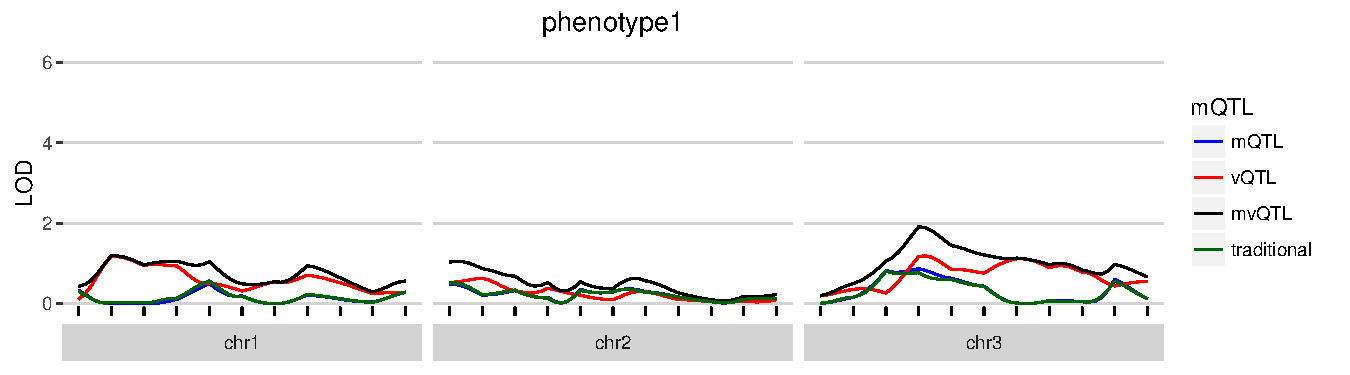
\includegraphics[width=\textwidth]{images/LOD_scan_phenotype1.pdf}
    \end{subfigure}

    \begin{subfigure}[b]{0.5\textwidth}
        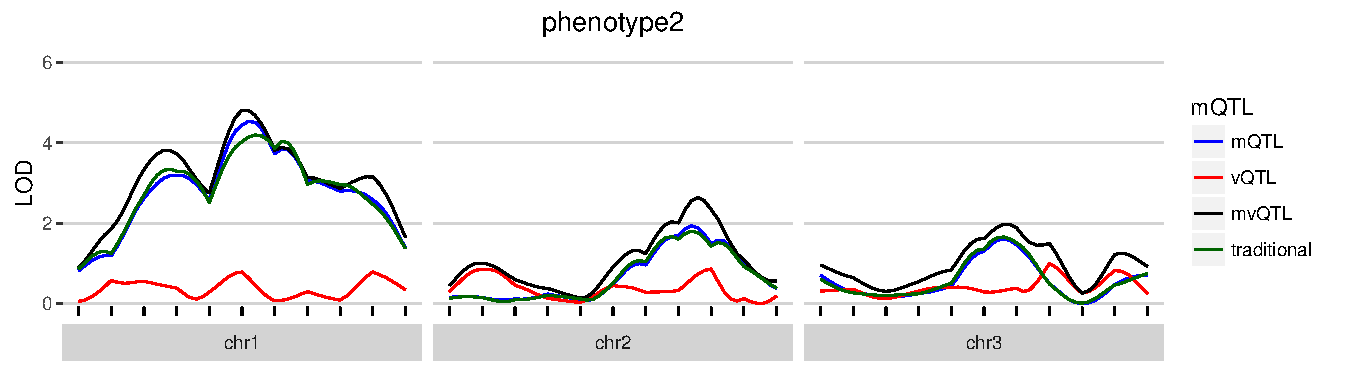
\includegraphics[width=\textwidth]{images/LOD_scan_phenotype2.pdf}
    \end{subfigure}

    \begin{subfigure}[b]{0.5\textwidth}
        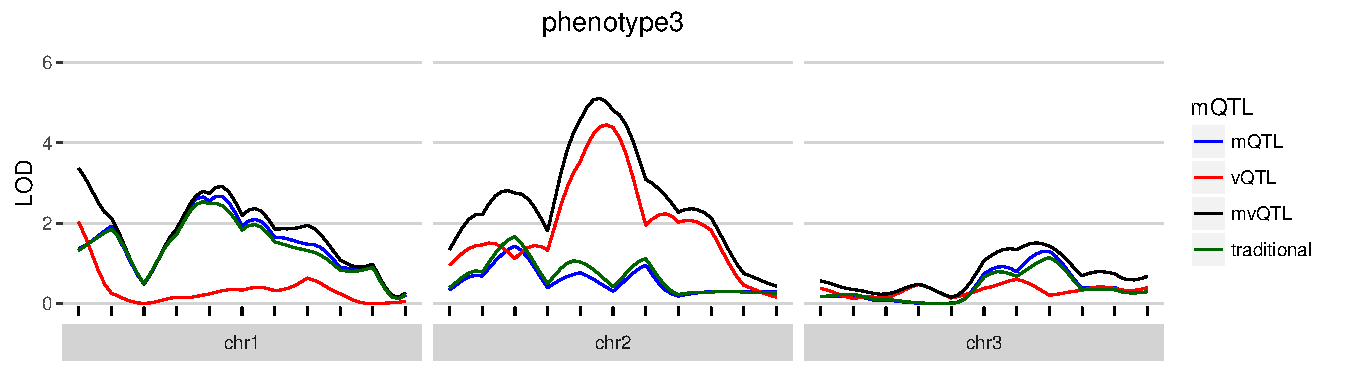
\includegraphics[width=\textwidth]{images/LOD_scan_phenotype3.pdf}
    \end{subfigure}
    
    \begin{subfigure}[b]{0.5\textwidth}
        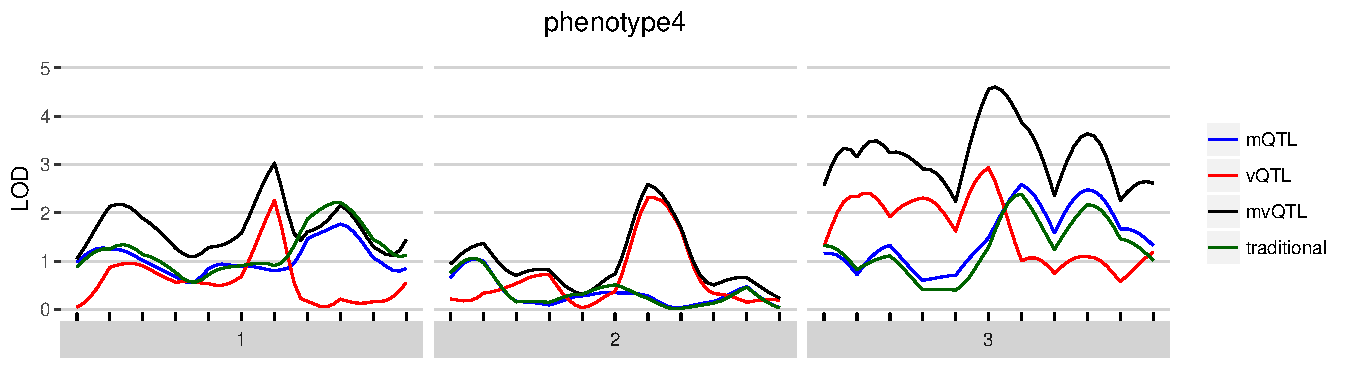
\includegraphics[width=\textwidth]{images/LOD_scan_phenotype4.pdf}
    \end{subfigure}
    
    \caption{For each of the four simulated phenotypes, the genome scan shows the LOD score of each test -- mean, variance, and joint -- in blue, red, and black, respectively.  The traditional test is in green and globally similar to the mean test. \label{fig:lod_score_scans}}
\end{figure}


The LOD score is the traditional test statistic in QTL mapping, but its interpretation can be difficult for two reasons:
1) LOD scores must be interpreted differently in autosomes and sex chromosomes.  The sex chromosomes are typically fit with fewer parameters, so the LOD scores are typically lower.
2) LOD scores from different tests must be interpreted differently.  For example, the LOD score of the mvQTL test is always higher than the LOD score of the mQTL and vQTL tests, because they are nested tests.

These difficulties in interpreting the LOD score are borne out in figure~\ref{fig:lod_score_scans}.
Given the scale of the vertical axis, it seems that there are no important signicals in the genome scan of \texttt{phenotype1}.
It is visually clear that the most interesting signals for \texttt{phenotype2}, \texttt{phenotype3}, and \texttt{phenotype4} are on chromosomes one two and three, respectively.
But it is not evident how to compare the results of the mvQTL test to the results of the other tests.
Nor would it be clear how to compare the results of tests from sex chromosomes, if they were present, to those from autosomes.
Nor is is possible to make an appropriate multple testing correction to account for the many tests that are conducted in a genome scan.

To put all genetic loci and all three tests on a level playing field, we consider two types of $p$-values:
1) Asymptotic $p$-values are calculated by \texttt{scanonevar} using the $\chi^2$ distribution with the appropriate degrees of freedom.  Though these $p$-values overcome the two problems of working with LOD scores described above, they leave unresolved the problem of interpreting $p$-values when many tests were conducted.
2) Empirical, family-wide error rate (FWER) -corrected $p$-values resolve the multiple-testing issue, thus they are the recommended means of assessing the significance of QTL mapping results.  Methods for calculating them are described in the next section.

The object returned by the \texttt{scanonevar} function has class \texttt{scanonevar}.
Calling \texttt{plot} on this object produces a publication-quality plot that shows the three association statistics at each locus.
Calling \texttt{summary} on this object produces a summary of how the scan was conducted and what the results were.





\section*{Assess the Significance of Results}


The effective number of statistical tests conducted in a family of tests (a genome scan) typically must be estimated to control family-wide error rate (FWER).
The effective number of tests in a genome scan, however, is difficult to estimate.
One lower bound is the number of chromosomes.
Due to the randomization in meiosis no two non-syntenic loci are correlated in an experimental cross and therefore tests on different chromosomes are always independent.
But there are many tests conducted on each chromosome, so the number of chromosomes is an under-estimate.
One upper bound on the effective number of tests is the total number of loci.
But, loci on the same chromosome are often in linkage disequilibrium, therefore the tests are not independent and the total number of loci is an over-estimate.

Our empirical approach sidesteps estimation of the effective number of tests.
We conduct many genomes scans, each executing a carefully-constructed model comparison to maintain all mean and variance effects of covariates and any non-focal genetic effects on mean and variance.
The details of these model comparisons are provided in the companion article.
For each test, we extract the highest observed value of the test statistic from each permutation scan and use those to model a generalized extreme value distribution.
The observed LOD scores from the genome scan are then transformed by the cumulative distribution function of the extreme value distribution to estimate the FWER-controlling $p$-values.
This approach is implemented in \texttt{scanonevar.perm}.
\texttt{scanonevar.perm} takes two required inputs:

\begin{enumerate}
	\item \texttt{sov} is the \texttt{scanonevar} object, the statistical significance of which will be assessed through permutation.
	\item \texttt{n.perms} is the number of permutations to conduct.
\end{enumerate}

The object returned by \texttt{scanonevar.perm} is a \texttt{scanonevar} object with one important additional piece of information, an empirical $p$-value for each test at each locus.
These $p$-values are FWER-corrected, so a value of $0.05$ for a specific test at a specific locus implies that in 5\% of similar experiments where there is no true genotype-phenotype association, we would expect to observe \textit{some} locus this significant or more significant.
A list of the per-genome-scan maximum observed LOD for each test and each chromosome type.


\begin{figure}[ht!]
    \begin{subfigure}{0.5\textwidth}
        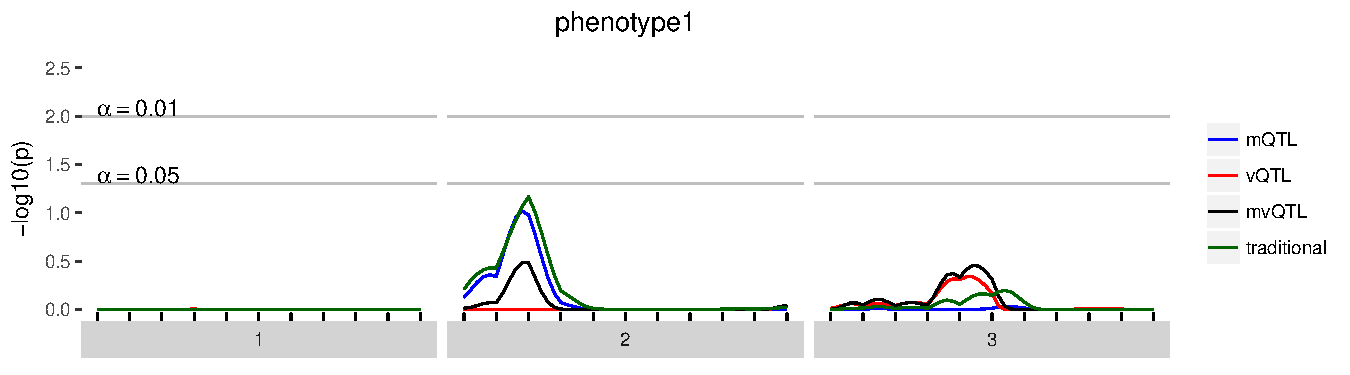
\includegraphics[width=\textwidth]{images/empir_p_scan_phenotype1.pdf}
    \end{subfigure}

    \begin{subfigure}[b]{0.5\textwidth}
        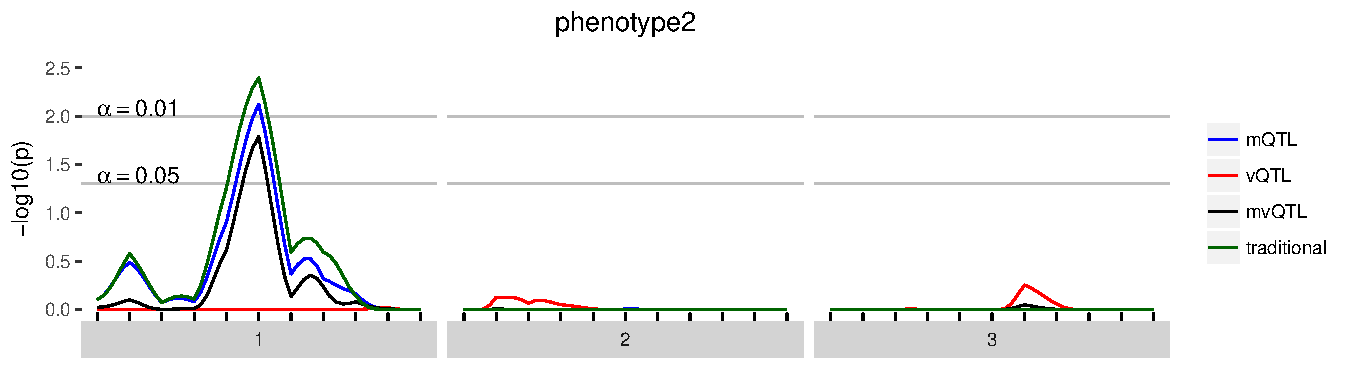
\includegraphics[width=\textwidth]{images/empir_p_scan_phenotype2.pdf}
    \end{subfigure}

    \begin{subfigure}[b]{0.5\textwidth}
        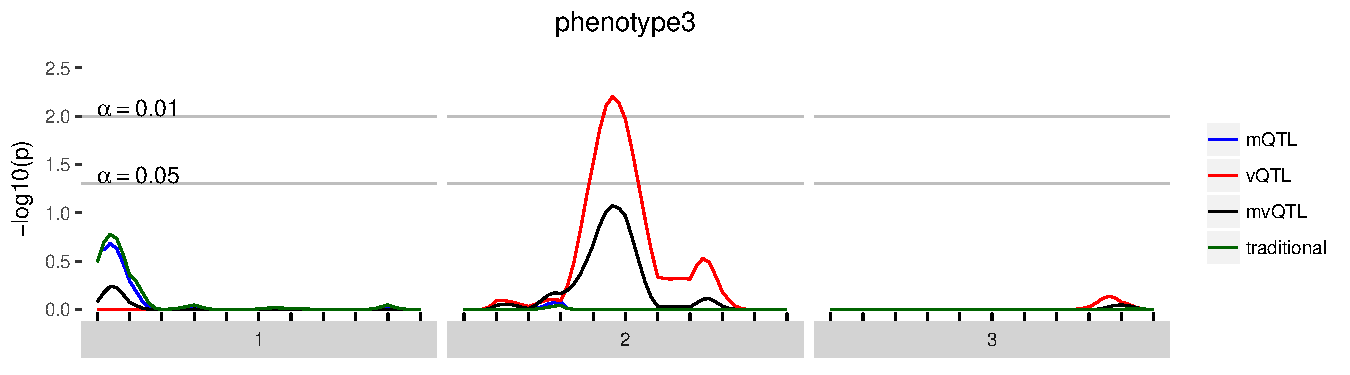
\includegraphics[width=\textwidth]{images/empir_p_scan_phenotype3.pdf}
    \end{subfigure}
    
    \begin{subfigure}[b]{0.5\textwidth}
        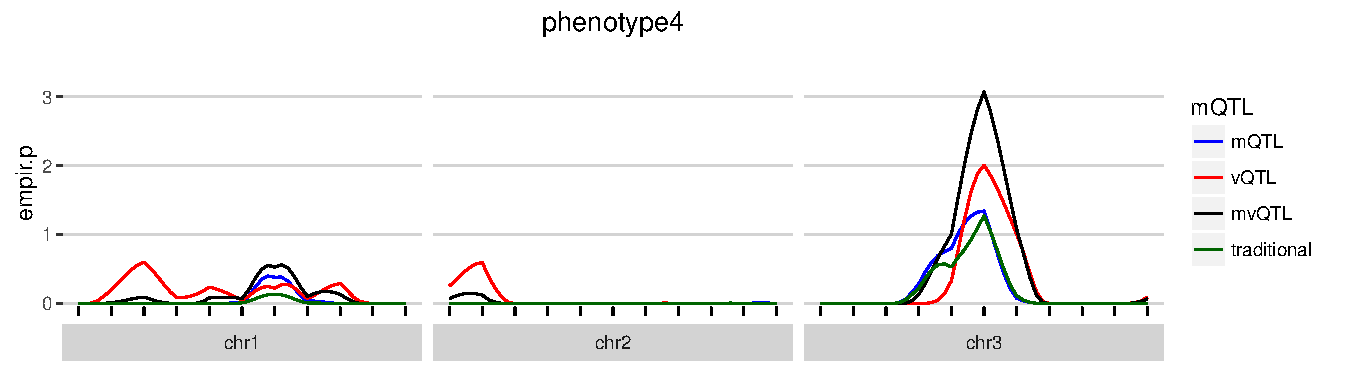
\includegraphics[width=\textwidth]{images/empir_p_scan_phenotype4.pdf}
    \end{subfigure}
    
    \caption{For each of the four simulated phenotypes, the genome scan shows the -log10 of the FWER-corrected $p$-value of each test -- mean, variance, and joint -- in blue, red, and black, respectively. Thus, a value of 3 implies that the quantity of evidence against the null is such that we expect to see this much or more evidence once per thousand genome scans when there is no true effect. \label{fig:empir_p_scans}}
\end{figure}


Accurate estimation of the FWER-controlled $p$-values requires many permutation scans.
We recommend at least 100, and rarely more than 1000.
These permutation scans can be run on multiple processors by specifying the optional \texttt{n.cores} argument.
On an Intel Core i5, running 100 permutations takes about five minutes.
When many phenotypes are studied, or the 5-50 minute runtime is problematic, these permutation scans can be broken into groups with different values for \texttt{random.seed}, run on separate computers, and combined with the \texttt{c} function.
This function combines the permutations from all the inputted scans, re-evaluates the observed LOD scores in light of all available permutations, and returns a new \texttt{scanonevar} object with more precisely estimated empirical $p$-values in about one second.






\section*{Investigate Significant Findings}

\begin{figure}[htbp]
    \begin{subfigure}[t]{0.24\textwidth}
        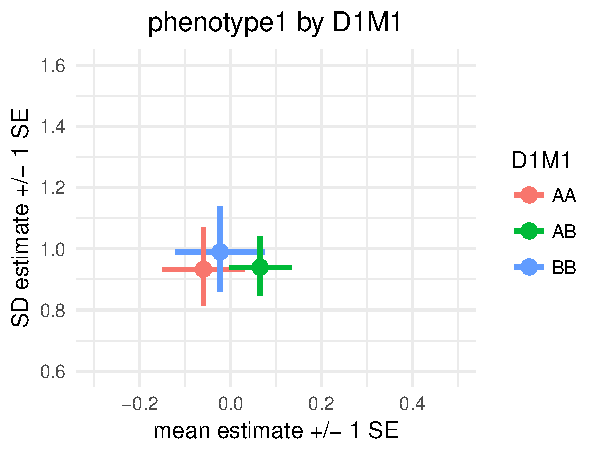
\includegraphics[width=\textwidth]{images/mean_var_plot_phen1.pdf}
    \end{subfigure}
    \hfill
    \begin{subfigure}[t]{0.24\textwidth}
        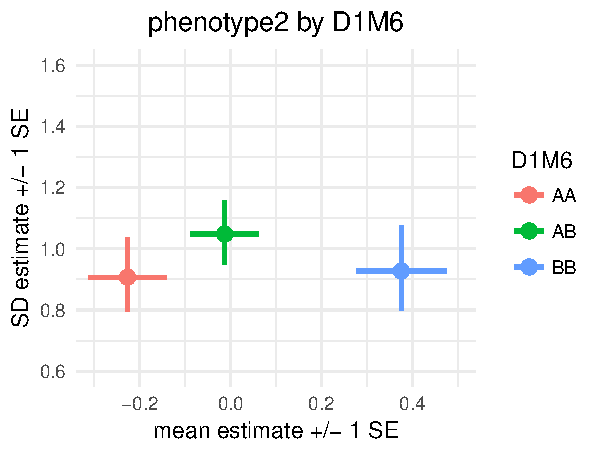
\includegraphics[width=\textwidth]{images/mean_var_plot_phen2.pdf}
    \end{subfigure}

    \begin{subfigure}[t]{0.24\textwidth}
        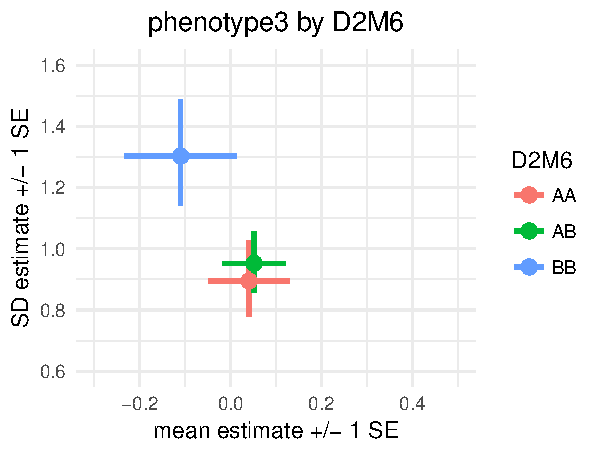
\includegraphics[width=\textwidth]{images/mean_var_plot_phen3.pdf}
    \end{subfigure}  
    \hfill
    \begin{subfigure}[t]{0.24\textwidth}
        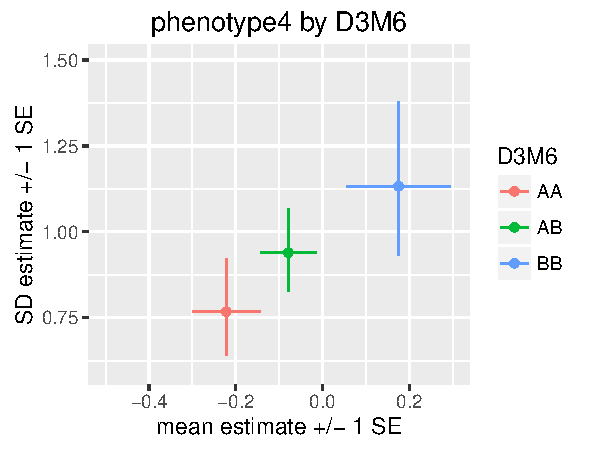
\includegraphics[width=\textwidth]{images/mean_var_plot_phen4.pdf}
    \end{subfigure}
    
    \caption{mean\_var plots show the estimated genotype effects at a locus, with mean effects on the horizontal axis and variance effects on the vertical axis.  Horizontal lines indicate standard errors for mean effects and vertical lines indicate standard errors for variance effects.  More information on the interpretation of these plots is provided in the `Investigate Significant Findings' section. \label{fig:mean_var_plots}}
\end{figure}

Having identified some QTL, we want to visualize the allele effects at those loci.
Because the \texttt{vqtl} package models both mean and variance effects, existing plotting utilities aren't able to display the entirety of the modeling results.
To investigate the results of a \texttt{vqtl} scan at one particular locus, we developed the \texttt{mean\_var\_plot}.
This plot shows information about the phenotype mean on the horizontal axis and information about the phenotype variance on the vertical axis.
There are both ``model-free'' and ``model-based'' versions of this plotting utility, but here we show only the ``model-based'' version for conciseness.

Figure~\ref{fig:mean_var_plots} shows a model-based \texttt{mean\_var\_plot} for each of the four phenotypes.
In each plot, the location of the dot shows the estimated mean and variance effect of each genotype, with the mean effect indicated by the horizontal position and the variance effect indicated by the vertical position.
The horizontal lines extending to the left and right from each dot show the standard error of the mean estimate, and the vertical lines extending up and down from each dot show the standard error of the variance estimate.
Additional grouping factors, such as sex, treatment group, or batch can also be specified and all combinations of effects for which an observation was made are plotted, but we here we show only the allele effects for clarity.

For phenotype1, the \texttt{mean\_var\_plot} is shown at the first marker of the first chromosome.
The estimates of the genotype effects on phenotype mean and variance are within one standard error of each other.
This pattern is consistent with the fact that there are no genetic effects, and the $p$-value was not statistically significant at any locus.

For phenotype2, the \texttt{mean\_var\_plot} is shown at the most significant marker, the tenth marker on the first chromosome.
The estimates of the genotype effects differ in the horizontal axis, but not the vertical axis.
This pattern is consistent with the fact that there is a genetic effect on phenotype mean but none on phenotype variance and with the highly significant $p$-value for the mQTL test, but non-significant $p$-value for the vQTL test.

For phenotype3, the \texttt{mean\_var\_plot} is shown at the most significant marker, the tenth marker on the second chromosome.
The estimates of the genotype effects differ in the vertical axis, but on on the horizontal axis.
This pattern is consistent with the fact that there is a genetic effect on phenotype variance but none on phenotype mean and with the highly significant $p$-value for the vQTL test but non-significant $p$-value for the mQTL test.

For phenotype4, the \texttt{mean\_var\_plot} is shown at the most significant marker, the tenth marker on the third chromosome.
The estimates fo the genotype effects differ in both the horizontal and vertical axes.
This pattern is consistent with the fact that there is a genetic effect on both phenotype mean and variance and with the highly significant $p$-value for the mvQTL test and the marginally significant $p$-values for the other two tests.






\section*{Conclusion}

We have demonstrated typical usage of the new \texttt{vqtl} \texttt{R} package for QTL mapping in experimental crosses.
This package is most appropriate for crosses and phenotypes where nuisance covariates or genetic factors are known or suspected to influence phenotype variance.
In the case of genetic factors, they can be mapped.
In the case of nuisance covariates, they can be accommodated.

The central function of this package, \texttt{scanonevar}, carries out the initial genome scan.
The permutation function, \texttt{scanonevar.perm}, executes a carefully-constructed set of permutations to empirically estimate a FWER-controlling $p$-value for each observed LOD score.
A suite of plotting functions, e.g. the \texttt{mean\_var\_plot}, allows geneticists to evaluate the allelic and covariate effects that underlie detected signals.




\bibliography{10_Aim1-2016_G3_PackageVQTL}

\newpage
\section*{Appendix}

\begin{figure}[ht!]
    \begin{subfigure}{0.5\textwidth}
        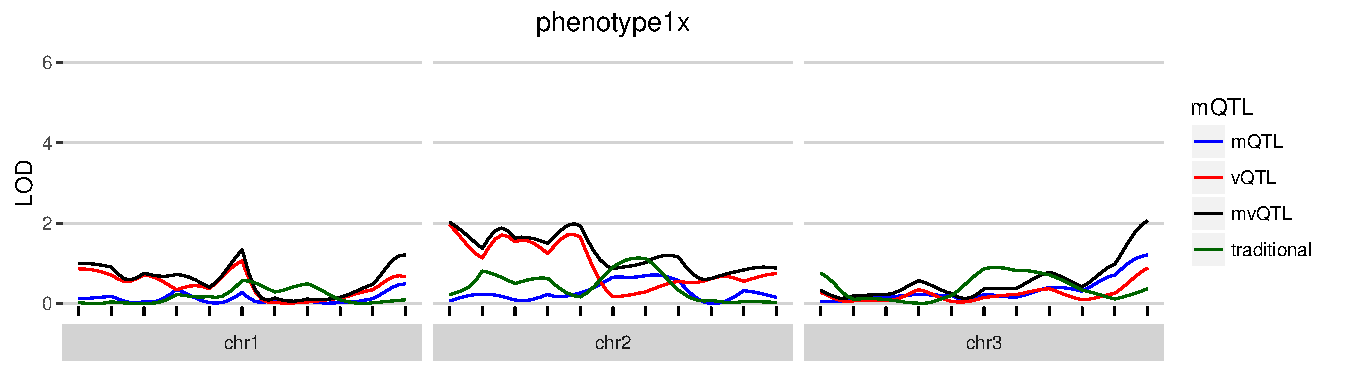
\includegraphics[width=\textwidth]{images/LOD_scan_phenotype1x.pdf}
    \end{subfigure}

    \begin{subfigure}[b]{0.5\textwidth}
        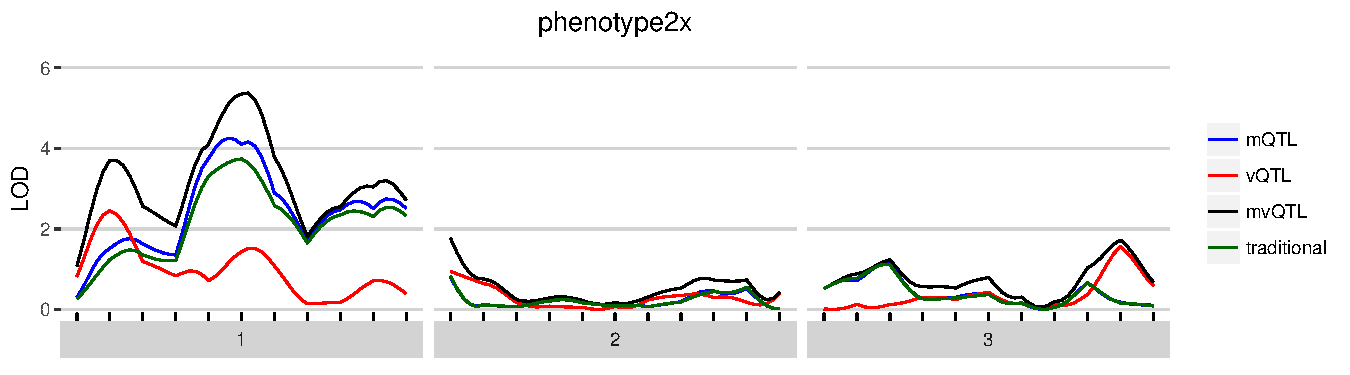
\includegraphics[width=\textwidth]{images/LOD_scan_phenotype2x.pdf}
    \end{subfigure}

    \begin{subfigure}[b]{0.5\textwidth}
        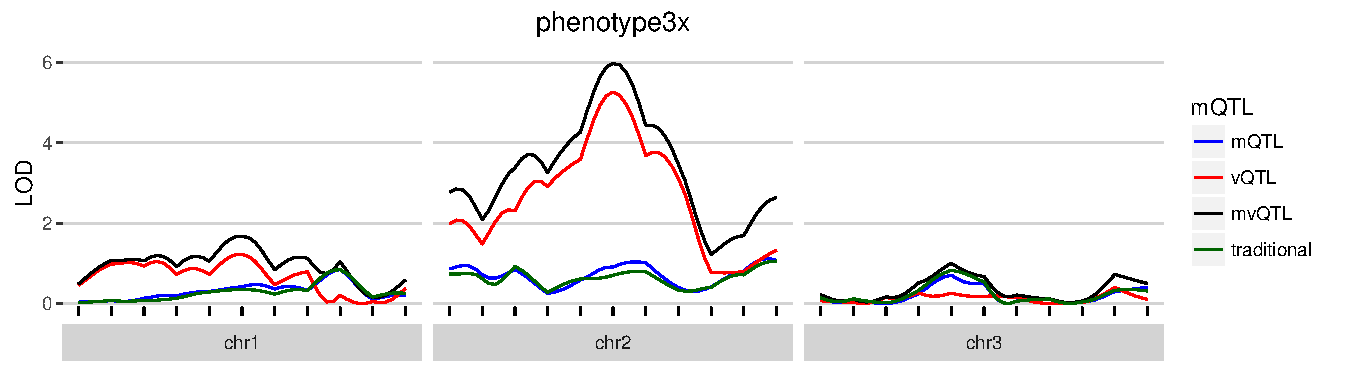
\includegraphics[width=\textwidth]{images/LOD_scan_phenotype3x.pdf}
    \end{subfigure}
    
    \begin{subfigure}[b]{0.5\textwidth}
        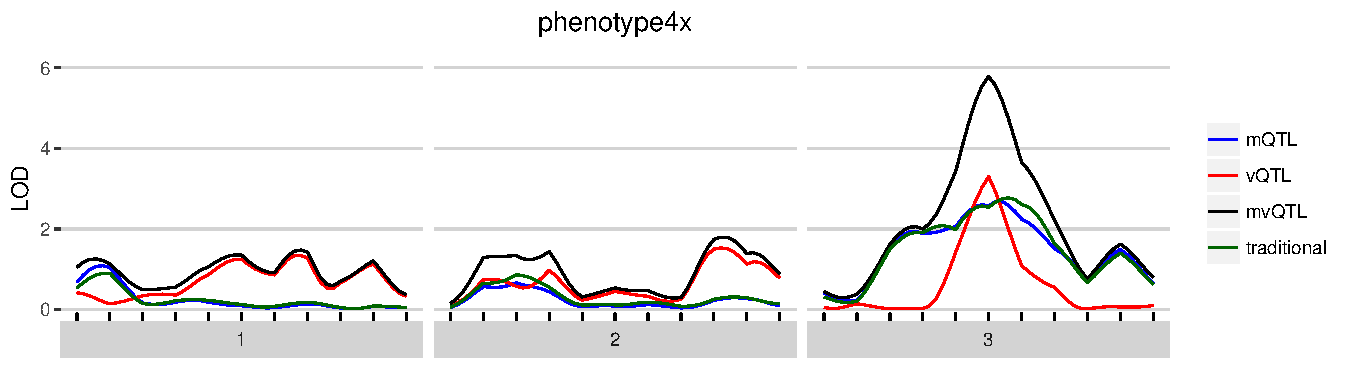
\includegraphics[width=\textwidth]{images/LOD_scan_phenotype4x.pdf}
    \end{subfigure}
    
    \caption{For each of the four simulated phenotypes, the genome scan shows the LOD score of each test -- mean, variance, and joint -- in blue, red, and black, respectively.  The traditional test is in green and globally similar to the mean test. \label{fig:apdx_lod_score_scans}}
\end{figure}



\begin{figure}[ht!]
    \begin{subfigure}{0.5\textwidth}
        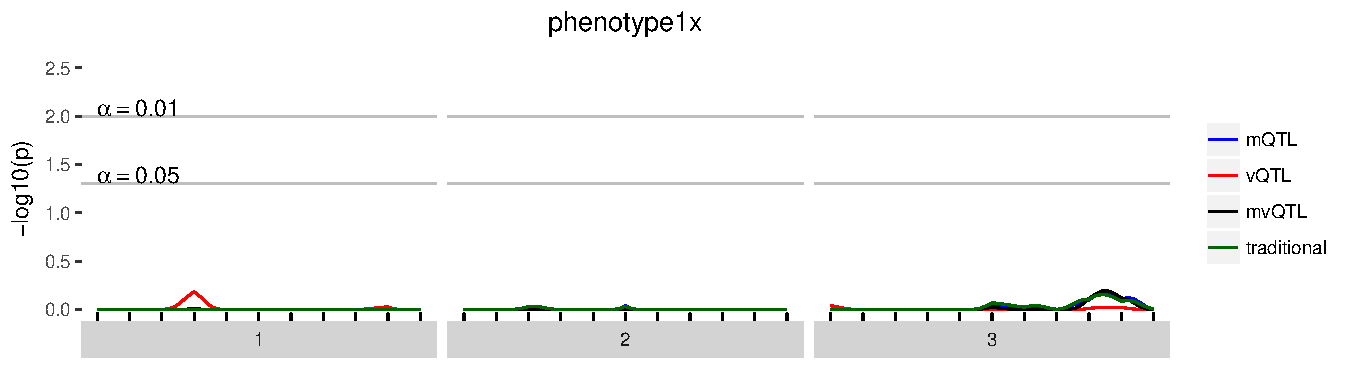
\includegraphics[width=\textwidth]{images/empir_p_scan_phenotype1x.pdf}
    \end{subfigure}

    \begin{subfigure}[b]{0.5\textwidth}
        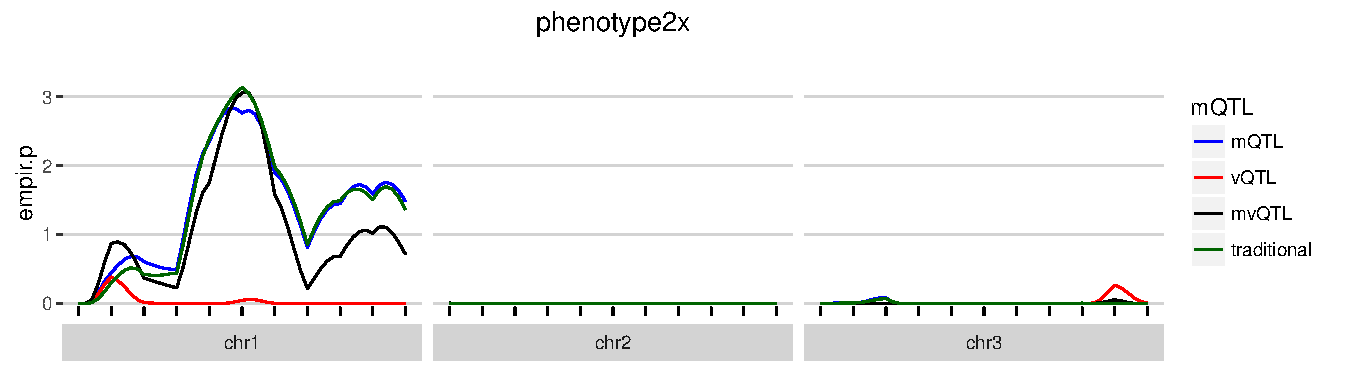
\includegraphics[width=\textwidth]{images/empir_p_scan_phenotype2x.pdf}
    \end{subfigure}

    \begin{subfigure}[b]{0.5\textwidth}
        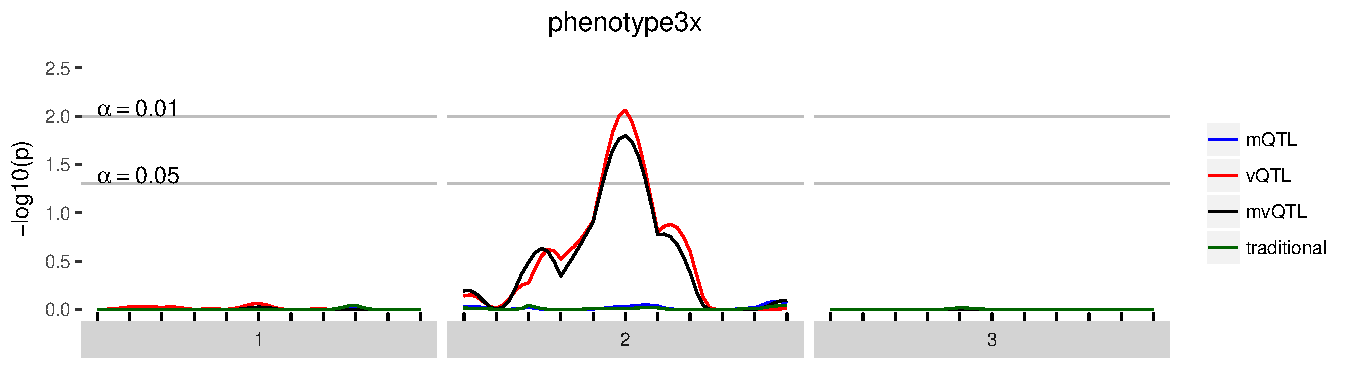
\includegraphics[width=\textwidth]{images/empir_p_scan_phenotype3x.pdf}
    \end{subfigure}
    
    \begin{subfigure}[b]{0.5\textwidth}
        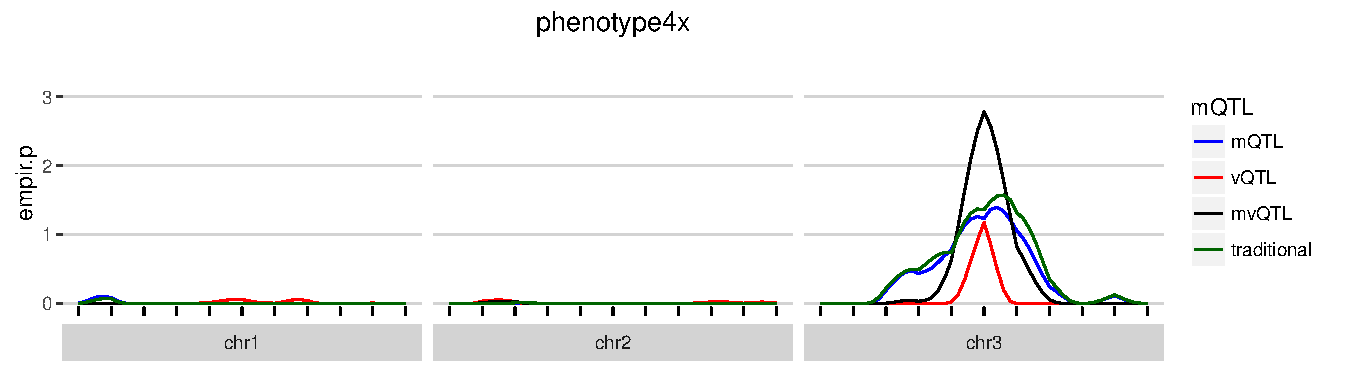
\includegraphics[width=\textwidth]{images/empir_p_scan_phenotype4x.pdf}
    \end{subfigure}
    
    \caption{For each of the four simulated phenotypes, the genome scan shows the -log10 of the FWER-corrected $p$-value of each test -- mean, variance, and joint -- in blue, red, and black, respectively. Thus, a value of 3 implies that the quantity of evidence against the null is such that we expect to see this much or more evidence once per thousand genome scans when there is no true effect. \label{fig:apdx_empir_p_scans}}
\end{figure}


\begin{figure}[htbp]
    \begin{subfigure}[t]{0.24\textwidth}
        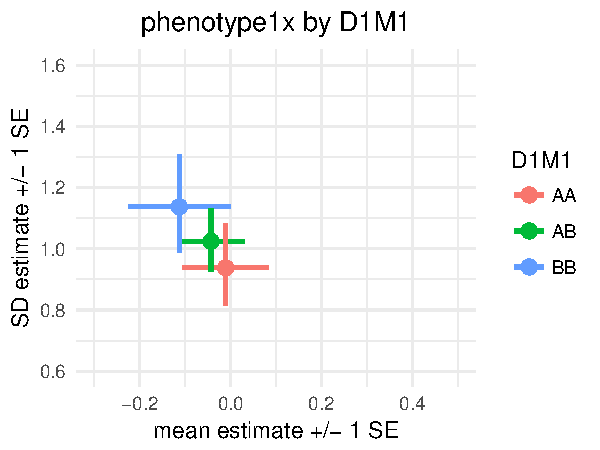
\includegraphics[width=\textwidth]{images/mean_var_plot_phen1x.pdf}
    \end{subfigure}
    \hfill
    \begin{subfigure}[t]{0.24\textwidth}
        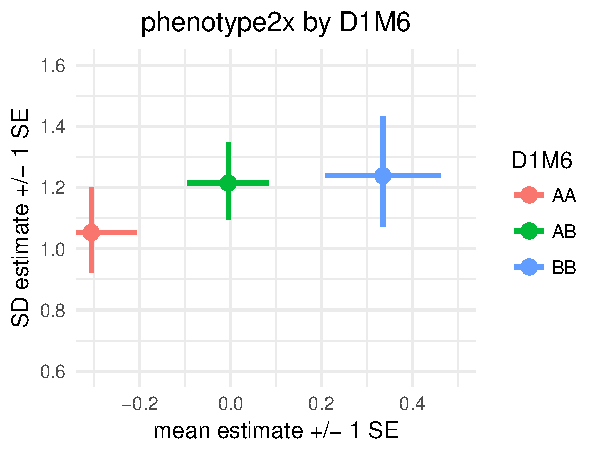
\includegraphics[width=\textwidth]{images/mean_var_plot_phen2x.pdf}
    \end{subfigure}

    \begin{subfigure}[t]{0.24\textwidth}
        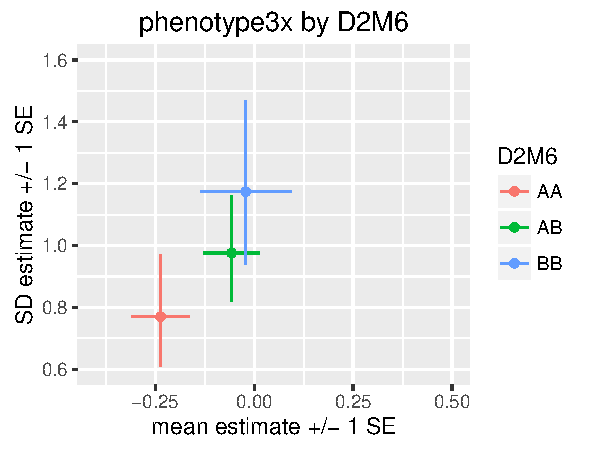
\includegraphics[width=\textwidth]{images/mean_var_plot_phen3x.pdf}
    \end{subfigure}  
    \hfill
    \begin{subfigure}[t]{0.24\textwidth}
        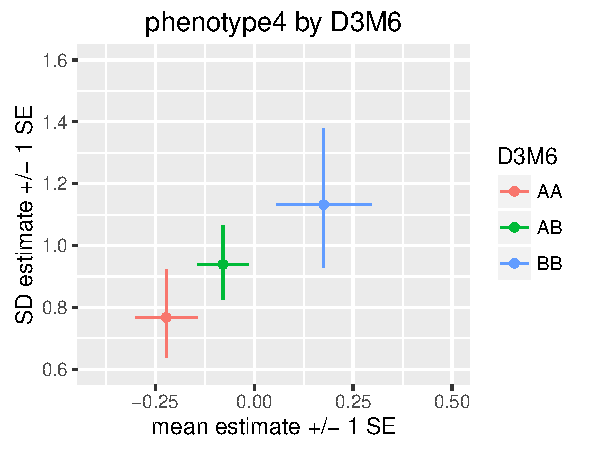
\includegraphics[width=\textwidth]{images/mean_var_plot_phen4x.pdf}
    \end{subfigure}
    
    \caption{mean\_var plots show the estimated genotype effects at a locus, with mean effects on the horizontal axis and variance effects on the vertical axis.  Horizontal lines indicate standard errors for mean effects and vertical lines indicate standard errors for variance effects.  More information on the interpretation of these plots is provided in the `Investigate Significant Findings' section. \label{fig:apdx_mean_var_plots}}
\end{figure}

\end{document}